\chapter{Progettazione di sistemi web}\label{ch:web}
  Il World Wide Web ha assunto un ruolo sempre più centrale nella quotidianità delle persone e nelle dinamiche di business.
  In particolare, il modello di comunicazione è sempre più virato verso scenari distribuiti,
  nei quali piattaforme eterogenee riescono a comunicare tra loro condividendo informazioni di diverso tipo attraverso la rete internet.

  Anche i pattern di progettazione e le tecnologie implementative sono cresciute altrettanto velocemente negli ultimi anni, cambiando anche radicalmente gli approcci di interazione possibili.
  Risulta dunque importante prestare attenzione allo stato dell'arte in tal senso, chiarendo quali siano i pattern più adatti e moderni per il contesto d'uso di questa tesi.

  \section{Architetture \& paradigmi}\label{sec:web-architecture}

  Con \emph{sistema web} si intende genericamente un sistema software distribuito che coinvolge una o più entità server che espongono in rete API di varia natura, con le quali entità client possono comunicare per usufruire dei servizi.
  Generalmente, in contesto web i client sono costituiti da pagine web aperte nei browser degli utenti.

  Le possibilità di progettazione di un'applicazione web possono essere molto differenti e nel tempo si è vista una vera e propria evoluzione in tal senso.

  % \begin{enumerate}
  %   \item
  %     Nel periodo iniziale del web, ciascuna pagina web era inviata al client come un documento statico;
  %     l'interazione dell'utente con il sistema avveniva attraverso la navigazione, che comportava l'apertura di una sequenza di pagine a seconda delle esigenze.
  %     Questo tipo di interazione era però lenta, in quanto coinvolgeva sempre la ricezione di una nuova pagina dal server.
  %   \item
  %     Successivamente, nel 1995, con l'introduzione da parte di NetScape di JavaScript (di cui tratteremo meglio nella~\Cref{subsec:js}) come linguaggio di scripting client-side, i programmatori hanno avuto la possibilità di inserire elementi dinamici nelle pagine web.
  %     In questo modo, era possibile effettuare alcune operazioni anche localmente, riducendo di fatto il numero di pagine intere scambiate con il server.
  %   \item
  %     Un'ulteriore innovazione apparve l'anno seguente, quando Macromedia introdusse \emph{Flash}:
  %     esso era un plugin per i browser che permetteva di riprodurre animazioni vettoriali e gestire le interazioni con l'utente, in modo simile a quanto fatto da JavaScript.
  %   \item
  %     Il termine ``\emph{web application}'' nasce però con l'introduzione della versione 2.2 della Java Servlet Specification~\cite{java1999specification} nel 1999.
  %     anche in questo caso, però, il server ha un ruolo centrale e ancora il concetto di \emph{ajax} (\emph{Asynchronous JavaScript + XML}) non è stato introdotto.
  %   \item
  %     Successivamente vi sono stati diversi miglioramenti incrementali, fino ad arrivare allo standard HTML5~\cite{Smith2008}:
  %     quest'ultimo, infatti, introduce il supporto nativo ai contenuti multimediali ed arricchisce la semantica del documento, oltre a migliorare l'integrazione con JS\@.
  %     Con questo standard, diventa sempre più comune il concetto di \emph{Single-page application} (SPA), secondo il quale la pagina viene caricata una sola volta, e poi modificata dinamicamente tramite chiamate specifiche al server.
  %     Nascono numerosi framework client-side (come Angular, Ember o React) e l'impiego del server viene sempre più circoscritto al fornire API per accesso controllato ai dati (ad esempio, un database) o per computazioni complesse.
  % \end{enumerate}

  Nel periodo iniziale del web, ciascuna pagina era inviata al client come documento statico;
  in questo caso, i server si occupavano della computazione di quanto richiesto dall'utente (anche appoggiandosi a servizi esterni tramite \emph{Common Gateway Interface}~\cite{Coar2004}) e della composizione del documento.

  Nel corso degli anni, sono stati sviluppati linguaggi di scripting (come JavaScript e Macromedia Flash) in grado di aumentare le possibilità di interazione lato client, riducendo la quantità di dati trasferiti tra il server web e il browser:
  non viene infatti più scaricata una nuova pagina ad ogni azione dell'utente, bensì solo i dati richiesti tramite chiamate \emph{AJAX} (\emph{Asynchronous JavaScript And XML});
  il documento viene poi manipolato localmente inserendo i dati ricevuti.

  Con l'avvento di HTML~5~\cite{Smith2008}, viene introdotto il supporto nativo ai contenuti multimediali ed arricchita la semantica del documento;
  inoltre JavaScript riceve un supporto di prima classe e la necessità di plugin esterni come Flash diminuisce.

  Vengono sviluppati numerosi framework per la realizzazione di applicazioni costituite da una singola pagina (\emph{SPA}, \emph{Single-Page Application}), in grado di offrire l'esperienza d'uso di un applicativo desktop.
  Un applicazione web moderna normalmente è di questo tipo.

  \improvement[inline]{Dovrei aggiungere qualche immagine per ridurre l'effetto wall-of-text?}

  \improvement[inline]{
    Inizialmente avevo inserito una storia dell'evoluzione delle architetture client-side e \strong{server-side}, ma poi mi sono reso conto che risultava un po' fuori contesto e l'ho tolta.

    Ritenete invece che potesse avere il suo senso come background? Nel caso posso reintegrarla velocemente.
  }

  % % Se inizialmente il server web si occupava dell'intero processo di costruzione della pagina, un po' alla volta le operazioni da effettuare per l'invio si sono sempre più ridotte.

  % % \begin{figure}[htbp]
  % %   \centering
  % %   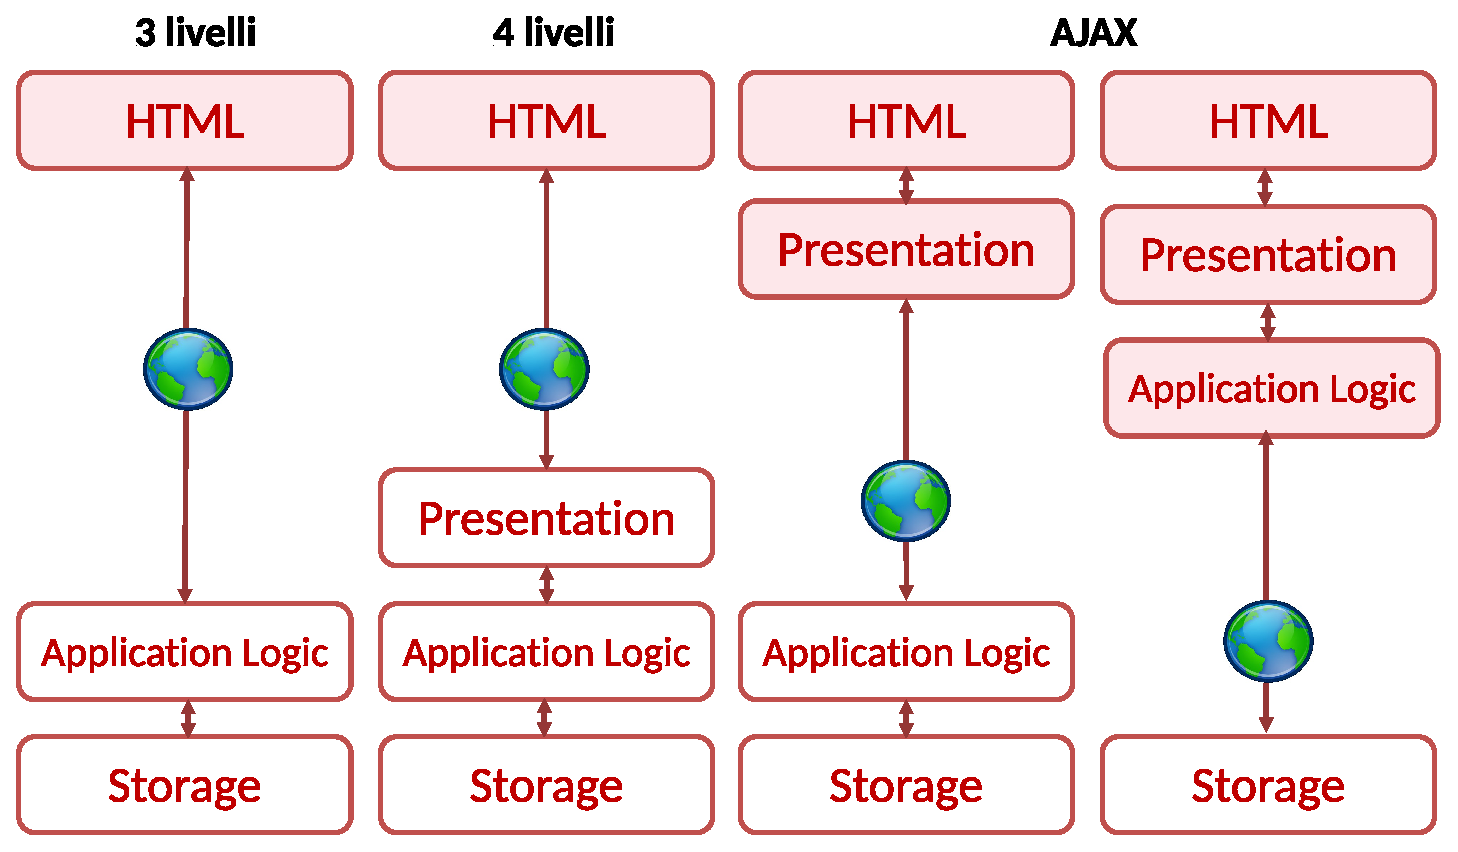
\includegraphics[width=.8\textwidth]{res/fig/server-evolution.eps}
  % %   \caption{Il controllo sulla costruzione della pagina si è spostato sempre più verso il client}%
  % %   \label{fig:server-evolution}
  % % \end{figure}

  % % In applicazioni l server diventa sempre più dedicato al memorizzare i dati (tramite database, ad esempio) e il codice client, mentre il browser si occupa di buona parte della logica applicativa.
  % Il primo approccio alla gestione della logica applicativa via rete fu quello di demandare la generazione dei contenuti a processi esterni tramite l'interfaccia standard CGI (\emph{Common Gateway Interface}~\cite{Coar2004}).
  % Essa permetteva al web server di lanciare un processo per ogni richiesta, passando i parametri necessari per l'elaborazione e di ricevere il risultato.
  % L'approccio era però poco scalabile e molto pesante per le risorse.

  \section{Linguaggi ad uso web}\label{sec:lang}
    In questa \nameCref{sec:lang} verranno analizzati i principali linguaggi di programmazione utilizzati recentemente per lo sviluppo della componente frontend delle applicazioni web.
    In particolare, verranno presi in considerazione i due linguaggi più popolari in questo contesto, ossia \emph{JavaScript} e il suo super-set \emph{TypeScript}, e due linguaggi provenienti da una diversa nicchia che possono offrire una valida alternativa: \emph{Scala.js} e \emph{Kotlin/JS}\@.

    \subsection{JavaScript e ECMAScript}\label{subsec:js}

      % \begin{wrapfigure}{r}{0pt}
      %   \centering
      %   % \vspace{-52pt}
      %   
\includegraphics[width=0.2\textwidth]{res/fig/js-logo.eps}
      %   % \vspace{50pt}
      %   \caption{Logo}%
      %   \label{fig:js}
      % \end{wrapfigure}

      \emph{JavaScript} è un linguaggio di scripting debolmente tipizzato multi-paradigma, con supporto agli stili di programmazione % funzionale, ad eventi, orientato agli oggetti.
      \begin{inparaitem}
        \item funzionale,
        \item ad eventi,
        \item orientato agli oggetti.
      \end{inparaitem}
      Sviluppato originariamente nel 1995 da Brendan Eich per Netscape Communications (inizialmente con il nome di \emph{Mocha} e poi \emph{LiveScript}),
      esso è stato concepito con lo scopo di avere un linguaggio di scripting per il browser Netscape Navigator più semplice da apprendere rispetto a quelli esistenti.
      JavaScript è stato standardizzato per la prima volta nel 1997 dalla ECMA con il nome di \emph{ECMAScript}~\cite{ECMA-262,ISO:1998} e l'attuale versione è la decima.

      Il linguaggio è attualmente il più popolare per uso web, in quanto l'unico ad essere supportato da tutti i browser moderni, almeno nelle sue feature principali.
      Diversi linguaggi, come quelli che vedremo in seguito, vengono transcompilati in una versione sufficientemente supportata di JS da poter essere eseguiti nei browser.

      Analizzato dal punto di vista tecnico, esso presenta i seguenti aspetti strutturali:

      \begin{description}
        \item[Imperativo e strutturato]
          Il linguaggio si presenta con una sintassi di programmazione strutturata standard, con il supporto a tutte le strutture di controllo tradizionali.
          Una parziale differenza era nella gestione della visibilità delle variabili (\emph{scope}):
          inizialmente, JavaScript garantiva solo la visibilità a livello di funzione (\emph{function scope}) tramite la parola chiave \texttt{var};
          con ECMAScript 6 è stato aggiunto il supporto alla visibilità a livello di blocco (\emph{block scope}).

        \item[Tipizzazione dinamica]
          % https://developer.mozilla.org/en-US/docs/Web/JavaScript/Data_structures
          JavaScript è un linguaggio debolmente tipizzato:
          alle variabili non sono associati dei tipi di dato, ma solo dei valori, che possono dinamicamente cambiare tipo durante il ciclo di vita della variabile.
          La tipizzazione dinamica consente lo stile di tipizzazione chiamato \emph{duck typing}~\cite{10.1145/2103621.2103686} (o \emph{structural subtyping}):
          è possibile determinare la semantica di un oggetto in base ai metodi ed alle proprietà che esso possiede,  non in base al suo tipo.

        \item[Orientamento agli oggetti Prototype-based]
          A differenza di altri linguaggi orientato agli oggetti (come Java o C++), JavaScript non fornisce un'implementazione del concetto di \emph{classe}~\cite{Ungar1991}:
          la stessa keyword \texttt{class}, introdotta con ES6, non è altro che zucchero sintattico per migliorare l'interazione da parte degli sviluppatori con il prototipo dell'oggetto.

          In termini di ereditarietà, infatti, JS prevede un solo costrutto: gli \emph{oggetti}.
          Ogni oggetto ha un collegamento interno ad un altro oggetto chiamato \emph{prototype}.
          Questo oggetto prototipo ha a sua volta un suo prototype, e così via finché si raggiunge un oggetto con la proprietà prototipo settata a \texttt{null}.
          Per definizione, \texttt{null} non ha un prototype ed agisce come anello finale nella \emph{catena di prototipi}.

          Quasi tutti gli oggetti in JavaScript sono istanze di \texttt{Object}, che risiede in cima alla catena dei prototipi.
          % In JavaScript, è possibile aggiungere proprietà a qualsiasi oggetto in fase di esecuzione.

        \item[First-class function]
          JavaScript offre un supporto di prima classe alle funzioni, che sono considerate oggetti;
          come tali, esse possono avere delle proprietà, come ad esempio \texttt{.bind()} e \texttt{.call()}. % ChkTeX 36

          Ciascuna funzione costituisce una chiusura lessicale.

          All'interno degli oggetti, le proprietà di tipo funzione vengono utilizzate come costruttori e come metodi.
          Infine, le funzioni possono essere utilizzate anche per l'implementazione di \emph{pattern di ruolo} come i \emph{tratti} e i \emph{mixin}.

        \item[Web APIs]
          Con ECMAScript si standardizza la componente \emph{core} del linguaggio, che può eseguire in ambienti browser come su interpreti non legati strettamente al web (come ad esempio Node.js~\cite{5617064}).
          Ciascuno degli ambienti nei quali il linguaggio viene interpretato mettono a disposizione delle API specifiche per l'interazione con la piattaforma;
          quando si fa riferimento al browser, tali supporti sono chiamati \emph{Web APIs}.

          Attraverso di esse, lo sviluppatore può avere accesso agli elementi del DOM (Document Object Model) di HTML, potendo manipolare la pagina visualizzata e reagire ad eventi su di essa.

        \item[Asincronismo]
          JavaScript supporta inoltre nativamente l'esecuzione di operazioni in modo asincrono tramite il costrutto della \emph{promise}, implementato da un oggetto built-in \texttt{Promise},
          che costituisce un \emph{proxy} per un valore non necessariamente noto quando la promise viene creata.
          È poi possibile gestire il valore ottenuto con costrutti ``\emph{thenable}'' o con il \emph{pattern async/await}.
      \end{description}

    \subsection{TypeScript}\label{subsec:ts}
      \emph{TypeScript} è un linguaggio di programmazione open-source sviluppato da Microsoft.
      Esso è un super-set sintatticamente rigoroso di JavaScript ES6, nato con i seguenti obiettivi principali:

      \begin{itemize}
        \item
          l'introduzione di funzionalità \emph{cutting-edge} (talvolta anche nei primi stage di approvazione) di ECMAScript.
          Esse sono rese disponibili transcompilando il sorgente TypeScript in codice JavaScript meno recentemente ma completamente compatibile con l'ambiente di esecuzione scelto
          (ad esempio ES5 per i browser), spesso avvalendosi di \emph{polyfill} per estendere la compatibilità.
          Tra queste funzionalità, ci sono ad esempio:
          \begin{description}
            \item[Decoratori]
              Definiti in una proposta ECMAScript~\cite{decorators} tutt'ora pendente (stage 2 al momento della scrittura),
              i decoratori sono dichiarazioni (definite tramite carattere ``\texttt{@}'') associate a una dichiarazione di classe, un metodo, una proprietà o un parametro che permettono la valutazione a runtime di una espressione specificata.
              Il framework Angular, ad esempio, utilizza estensivamente questa funzionalità per effettuare \emph{dependency injection}.

            \item[Operatore di coalescenza del null \& safe navigation]
              In JavaScript, sono considerati \emph{falsy} valori come \texttt{NaN}, \texttt{0} e la stringa vuota che, pur non essendo \texttt{null} o \texttt{undefined},
              vengono trattati come valori ``non presenti'' e dunque come \texttt{false} dagli operatori booleani.
              Per ridurre la possibilità di bug dovuto a questo tipo di valori, sono stati definiti gli operatori di \emph{nullish coalescing} ``\texttt{??}'' e di \emph{safe navigation} ``\texttt{.?}''.
              Definiti sulla base di una precedente proposta ECMAScript~\cite{optional}, solo più tardi integrata, sono stati introdotti con la versione 3.7.3 di TypeScript.
          \end{description}
        \item
          l'introduzione di un sistema di \emph{tipizzazione statica} opzionale che possa integrarsi nel modo più trasparente possibile nella sintassi JavaScript standard;
          in particolare, viene data la possibilità di definire tipi complessi tramite \emph{sintassi postfissa}.
      \end{itemize}

      % Di fatto, dunque, presenta tutte le caratteristiche di JavaScript descritte nella \Vref{subsec:js}.
      Il sistema di tipi viene presentato come \emph{class-based} (in contrapposizione al \emph{prototype-based} tipico di JavaScript, soprattutto prima dell'introduzione dello zucchero sintattico per le classi), ma mantiene le caratteristiche di structural subtyping citate precedentemente.
      Avvalendosi di ciò, il linguaggio permette la definizione di tipi complessi;
      è garantito il supporto ai generici, esteso da un'algebra dei tipi molto flessibile che permette unione, intersezione e condizionalità, oltre alla possibilità di accesso ai tipi delle singole proprietà.

      % Il linguaggio permette la definizione di interfacce che descrivono la struttura delle proprietà attese al compilatore.
      % Tali interfacce offrono la possibilità di definire tipi complessi:

      % \begin{description}
      %   \item[Tipi funzione]
      %     Tramite le interfacce è possibile definire le strutture di funzioni, che possono essere implementate in modo anonimo nel codice attraverso il costrutto \texttt{function} o ``\emph{fat arrow}'' (\texttt{=>}).
      %     % \inputminted{typescript}{res/code/functionType.ts}
      %   \item[Indexable Types]
      %     È possibile
      % \end{description}

      % \begin{itemize}
      %   \item \emph{tipi funzione}, che definiscono l'oggetto come una funzione di una determinata struttura;
      %   \item \emph{tipi indicizzabili}, che definiscono oggetti che possono fornire l'accesso a proprietà interne tramite \emph{bracket notation} (ad esempio, l'\texttt{Array});
      %   \item \emph{tipi ibridi}, con i quali è possibile interagire tramite differenti notazioni
      % \end{itemize}

      La generazione dei metadati per la descrizione dei tipi permette un'integrazione migliore di TypeScript e JavaScript con gli ambienti di sviluppo;
      inoltre, negli anni è diventato lo standard de-facto per la documentazione dei moduli per il linguaggio, sostituendo le soluzioni basate sul parsing dei commenti come JSDoc.

    \subsection{Scala.js}\label{subsec:scalajs}
      \emph{Scala.js} è un compilatore per il linguaggio di programmazione Scala che genera codice JavaScript invece di bytecode per la JVM\@.
      % Questo permette l'impiego di tutte le funzionalità di Scala in contesto web, massimizzando il riuso di codice condiviso con la componente backend potenzialmente scritto con il medesimo linguaggio e in esecuzione su JVM\@.

      I principali vantaggi dell'impiego di un linguaggio come Scala all'interno del contesto web sono i seguenti:
      \begin{description}
        \item[Struttura più solida]
          Come detto, JavaScript è un linguaggio debolmente tipizzato;
          se questo aggiunge notevole flessibilità durante lo sviluppo, d'altro canto aggiunge una maggiore possibilità di bug.
          Anche TypeScript, che offre un sistema di tipi molto più completo, risulta talvolta anomalo per via della natura strutturale della tipizzazione implementata.

          Scala mette a disposizione un type system allo stesso tempo più espressivo e più rigoroso, di conseguenza può risultare più \emph{user-friendly} sia durante lo sviluppo che in fase di debug.

        \item[Prestazioni]
          Secondo benchmark~\cite{Doeraene:256862} realizzati tramite una suite estensiva già utilizzata in letteratura~\cite{10.1145/3093334.2989232}, per quanto Scala.js risulti più lento della controparte JVM, riesce ad essere fino al 33\% più veloce della controparte scritta in JavaScript.

          Inoltre, il compilatore risulta molto efficiente in termini di dimensioni finali del \emph{bundle}:
          secondo il sito ufficiale, generalmente si parte dai \(\SI{45}{\kilo\byte}\) per un'intera applicazione compressa in gzip.
          Questo permette di avere buone performance al primo caricamento dell'applicazione web.

        % \item[Interoperabilità \& riuso]
        \item[Interoperabilità con JavaScript]
          % Un terzo vantaggio risiede nelle possibilità di interoperare con codice già esistente, sia con JavaScript che con Scala.
          % In particolare,
          Scala.js è dichiaratamente compatibile con qualsiasi modulo JavaScript, purché sia dotato del codice \emph{façade} necessario per garantirne il type checking.
          Il team che mantiene il progetto ha effettuato il wrapping di numerose librerie di uso comune (50 al momento della scrittura) e mette a disposizione uno strumento di conversione automatico per le definizioni di tipo generate dal compilatore di TypeScript.
          Data la popolarità di quest'ultimo, la copertura può essere dunque considerata elevata.

        \item[Riuso]
          Un'altra compatibilità utile nella realizzazione di sistemi web di grandi dimensioni è quella con codice Scala impiegato anche nel backend.
          Questo permette di riutilizzare il codice condiviso tra server e client,
          riducendo i costi di manutenzione del medesimo codice in linguaggi differenti e la possibile \emph{friction} originata dall'etereogeneità dei linguaggi.

          Non è possibile riutilizzare codice che dipende strettamente da funzionalità della JVM (\emph{reflection}, eccezioni native di Java), in quanto porta a comportamenti indefiniti.
      \end{description}

      % Oltre al supporto semi-ufficiale a React e altri framework e librerie per la realizzazione di SPA, Scala offre un'integrazione di prima classe anche con tecnologie backend molto famose come il Play Framework di Lightbend.
      Scala inoltre ha un'integrazione molto buona con ambienti di sviluppo comunemente utilizzati, che può portare a una rilevazione degli errori più veloce e ad un autocompletamento più preciso.

    \subsection{Kotlin/Multiplatform e Kotlin/JS}\label{subsec:kotlinjs}
      Con il rilascio della versione 1.1 di Kotlin nel 2017, JetBrains ha annunciato \emph{Koltin/JS}~\cite{Belov2017}, un target del compilatore in grado di generare codice JavaScript ES5 invece che bytecode per la JVM, in modo simile a quanto fatto da Scala.js.
      Il progetto si colloca in un progetto di più ampio respiro, ossia \emph{Kotlin/Multiplatform}~\cite{Jemerov2017}, presentato al termine dello stesso anno in concomitanza con Kotlin 1.2, che mira a integrare anche il supporto ad altri target, tra cui ad esempio LLVM\@.

      L'intento è molto simile a quello di Scala.js:
      fornire un linguaggio solido per la realizzazione di componenti web (ad esempio un frontend) con lo stesso codice in esecuzione sul server con cui dialogare, in modo da coprire l'intero sistema nel modo più omogeneo possibile.

      Kotlin, a differenza di quanto avviene in Scala.js, però, prevede l'utilizzo di sorgenti separati per la parte comune (\emph{common source set}), che modella il sistema in Kotlin puro, e per la parte specifica di ciascun particolare target:
      in questo modo, differenti piattaforme possono avere implementazioni più vicine alle rispettive native, avvalendosi di librerie specifiche fornite dal sistema o da terze parti.
      % Questo pattern è realizzato attraverso le parole chiave \texttt{expected} e \texttt{actual} anteposte alle definizioni che

      Anche in questo caso, le criticità sono simili a quelle citate nella \nameCref{subsec:scalajs} precedente:
      \begin{itemize}
        \item
          per quanto l'intera libreria standard sia stata portata da JetBrains sulle diverse piattaforme nel modo più trasparente possibile, le piattaforme di esecuzione rimangono differenti.
          Di conseguenza, alcuni costrutti molto specifici strettamente legati alla JVM (come ad esempio la reflection) non sono disponibili sul target JS\@.
        \item
          per garantire il supporto corretto ai tipi, è necessaria la presenza di codice \emph{wrapper} che li modelli.
          JetBrains ha realizzato gli adattamenti solo per poche librerie, principalmente legate a React, e ha messo a disposizione alcuni strumenti per la conversione delle definizioni di tipo di TypeScript.
          Purtroppo, la prima soluzione, \texttt{ts2kt}, è stata deprecata solo dopo qualche anno e il sostituto, \texttt{dukat}, al momento della scrittura non è ancora considerato stabile.

          In assenza dei wrapper, è comunque possibile lavorare con moduli JavaScript attraverso il costrutto \texttt{dynamic}, ma si perde il controllo sui tipi.
      \end{itemize}

      JetBrains pare supportare attivamente la libreria React per la realizzazione di codice frontend, ma attualmente non viene ritenuto ancora sufficientemente stabile per un uso reale.
      Sul sito ufficiale sono invece specificati numerosi framework per la realizzazione di backend che offrono supporto di prima classe al linguaggio.
